\chapter{Ground states, symmetries, and defects}
In this chapter we investigate the ground states of spinor BECs obtained through
minimizing the corresponding mean-field energy functional.
In particular, we investigate the symmetry properties using both Majorana and
spherical harmonic representations.
Furthermore, we construct the phase diagrams for conserved and non-conserved
magnetisation.
Finally, we construct some topological defects present in these systems.

There are numerous references (e.g., see~\cite{Ciobanu2000, Zhang2003,
Kawaguchi2012, StamperKurn2013}) that already provide most of these results,
but we reproduce them here to provide reference for subsequent chapters.
Furthermore, there are subtleties between the phase diagrams of spinor BECs
in the presence of conserved magnetisation that is not widely reported, so we
construct both phase diagrams (conserved and non-conserved) here to clarify
distinctions between the two.


\section{Spin-1}

\subsection{Ground states in a uniform system}

For a spin-1 system, the interacting part of the energy functional contains
two independent non-linear interaction terms (\textcolor{red}{See relevant
section constructing interacting Hamiltonian}), given by
\begin{equation}
    E_\mathrm{int} = \frac{1}{2}\int c_0n^2+c_1|\vb{F}|^2 d\vb{r}.
\end{equation}
Since the density term remains fixed for a given normalised ground state, the
spin magnitude is the only relevant term when computing the ground state.
For ferromagnetic interactions (\(c_1 < 0 \)), the energy is minimised when
the spin magnitude is maximised, i.e., \(|\vb{F}| = n\).
A representative spinor for a ferromagnetic ground state is then
\begin{equation}
    \zeta^\mathrm{FM} = \mqty(1 \\ 0 \\ 0).
\end{equation}
In the absence of a magnetic field, the energy of a given spinor is degenerate
with respect to a global \(U(1)\) phase \(e^{i\theta}\) and an \(SO(3)\) spin
rotation, parameterized by three Euler angles \(\alpha, \beta \),
and \(\gamma \).
A general spin rotation represents rotations around the \(z-y-z\) axes:
\(U(\alpha, \beta, \gamma) = e^{-i\alpha F_z}e^{-i\beta F_y}e^{-i\gamma F_z}\).
In explicit matrix form, this becomes
\begin{equation}
    U(\alpha, \beta, \gamma) = \mqty(
        e^{-i(\alpha + \gamma)}\cos^2\frac{\beta}{2} &
        -\frac{e^{-i\alpha}}{\sqrt{2}}\sin\beta &
        e^{-i(\alpha - \gamma)}\sin^2\frac{\beta}{2} \\
        \frac{e^{-i\gamma}}{\sqrt{2}}\sin\beta &
        \cos\beta &
        -\frac{e^{i\gamma}}{\sqrt{2}}\sin\beta \\
        e^{i(\alpha - \gamma)}\cos^2\frac{\beta}{2} &
        \frac{e^{i\alpha}}{\sqrt{2}}\sin\beta &
        e^{i(\alpha + \gamma)}\sin^2\frac{\beta}{2}
    ).
\end{equation}
The general ferromagnetic wave function is constructed by
\begin{equation}
    \psi^\mathrm{FM} = 
    \sqrt{n}e^{i\theta}U(\alpha, \beta, \gamma)\zeta^\mathrm{FM} = 
    \sqrt{n}e^{i(\theta - \gamma)}\mqty(
        e^{-i\alpha}\cos^2\frac{\beta}{2} \\
        \frac{1}{\sqrt{2}}\sin\beta \\
        e^{i\alpha}\sin^2\frac{\beta}{2}
        ).
\end{equation}

For polar interactions (\(c_1 > 0\)), the energy is minimised by having the
spin magnitude vanish \(|F|=0\).
A representative polar spinor is
\begin{equation}
    \zeta^\mathrm{P} = \mqty(0 \\ 1 \\ 0).
    \label{eq: EAP-spinor}
\end{equation}
Similar to the FM case, a general polar wave function is given by
\begin{equation}
    \psi^\mathrm{P} = 
    \sqrt{n}e^{i\theta}U(\alpha, \beta, \gamma)\zeta^\mathrm{P} = 
    \sqrt{n}e^{i\theta}\mqty(
        -\frac{e^{-i\alpha}}{\sqrt{2}}\sin\beta \\
        \cos\beta \\
        \frac{e^{i\alpha}}{\sqrt{2}}\sin\beta
        ).
\end{equation}
Thus, in the absence of a magnetic field, there are two ground states in a
spin-1 system: polar and ferromagnetic, depending on the sign of the
spin-dependent interaction term, \(c_1\).

The presence of an external magnetic field drastically changes the valid ground
states of the spin-1 system.
\begin{figure}[htb]
    \centering
    \begin{tikzpicture}
        \node[anchor=south west, inner sep=0] (sodium) at (0, 0)
        {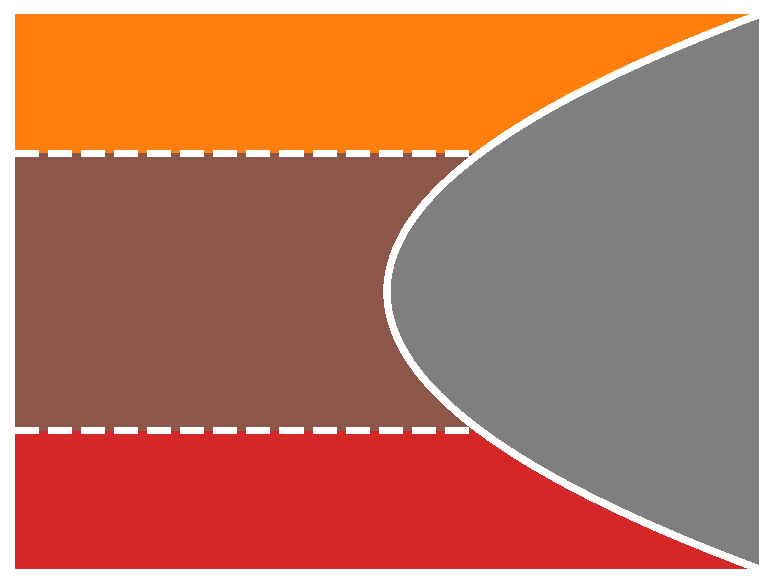
\includegraphics[width=0.38\textwidth]
        {gfx/ch-groundStateSymmetries/ground_states_polar_int_spin1.pdf}};
        \node[anchor=south west, inner sep=0] (rubidium) at (8, 0)
        {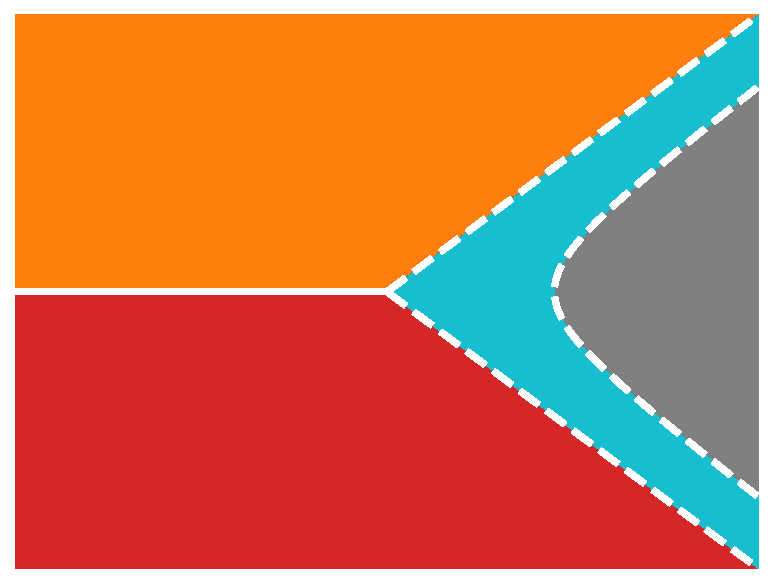
\includegraphics[width=0.38\textwidth]
        {gfx/ch-groundStateSymmetries/ground_states_fm_int_spin1.pdf}};
        
        \begin{scope}[x={($0.1*(sodium.south east)$)},
                      y={($0.1*(sodium.north west)$)}]
            \draw[->, thick] (0,5)--(10.3,5) node[right]{$\frac{q}{c_1n}$};
            \draw[->, thick] (4.97,0)--(4.97,10.3) node[above]{$\frac{p}{c_1n}$};
            \draw[-] (6.1, 4.8) -- (6.1, 5.2);
            \node[anchor = south west] at (6.5, 3)
            {\scriptsize $p^2=2c_1nq$};
            \draw[->, thick] (6.6, 3.1) -- (6.25,2.55);
            \node at (4.8, 7.75) {\scriptsize $1$};
            \node at (4.7, 2.25) {\scriptsize -$1$};
            \node at (6.1, 4.5) {\scriptsize 1/2};
            \node[anchor=south west] at (0.8, 8.2)
            {\textcolor{white}{Ferromagnetic (I)}};
            \node[anchor=south west] at (0.8, 0.5)
            {\textcolor{white}{Ferromagnetic (II)}};
            \node[anchor=south west] at (0.1, 4.9)
            {\textcolor{white}{\small Antiferromagnetic}};
            \node[anchor=south west] at (2.1, 3.8)
            {\textcolor{white}{(III)}};
            \node[anchor=south west] at (6.5, 4.9)
            {\textcolor{white}{Polar (IV)}};
            \node[anchor=south west] at (3.8, -1.5) {\large $c_1 > 0$};
        \end{scope}
        \begin{scope}[x={($0.1*(sodium.south east)$)},
            y={($0.1*(sodium.north west)$)}]
            \draw[->, thick] (18.9,5)--(24.2,5) node[right]{$\frac{q}{|c_1|n}$};
            \draw[->, thick] (18.9,0)--(18.9,10.3) node[above]
            {$\frac{p}{|c_1|n}$};
            \node[anchor=south west] at (18.8, 8.6) 
            {\scriptsize $p^2=q^2-2|c_1|nq$};
            \draw[->, thick] (19.3, 8.8) -- (21.5, 6.2);
            \node[anchor=south west, inner sep=0, rotate=-38] at (19, 4.2)
            {\scriptsize $p=-q$};
            \node[anchor=south west, inner sep=0, rotate=38] at (19.1, 5.3)
            {\scriptsize $p=q$};
            \node[anchor=south west, inner sep=0] at (21.2, 4.5)
            {\scriptsize $2$};
            \node[anchor=south west] at (14.8, 6.5)
            {\textcolor{white}{Ferromagnetic (I)}};
            \node[anchor=south west] at (14.8, 1.5)
            {\textcolor{white}{Ferromagnetic (II)}};
            \node[anchor=south west] at (19.7, 4.9)
            {\textcolor{white}{BA}};
            \node[anchor=south west] at (19.7, 3.8)
            {\textcolor{white}{(V)}};
            \node[anchor=south west] at (21.7, 4.9)
            {\textcolor{white}{Polar}};
            \node[anchor=south west] at (21.7, 3.8)
            {\textcolor{white}{(IV)}};
            \node[anchor=south west] at (18., -1.5) {\large $c_1 < 0$};
        \end{scope}
    \end{tikzpicture}
    \caption{\label{fig: GS-phase-diagram}Ground state phase diagrams of spin-1
    BECs for polar (\(c_1 > 0\)) and ferromagnetic (\(c_1 < 0\)) interactions
    in a parameter space of \((p, q)\).
    Solid or dashed white lines represent discontinuous and continuous phase
    transitions, respectively.}
\end{figure}
Fig.~\ref{fig: GS-phase-diagram} shows the ground state phase diagram for spin-1
BECs with \(c_1 > 0\) (left) and \(c_1 < 0\) (right) in the presence of a
magnetic field.
The full derivation of the ground state phase diagram can be found in recent
reviews~\cite{Kawaguchi2012, StamperKurn2013}.
There are five total ground states shown in Fig.~\ref{fig: GS-phase-diagram},
which are summarised in Table~\ref{tab: spin-1-ground-states}.
\begin{table}
    \centering
    \begin{tabular}{ccc}
        \toprule
        Ground state & Spinor, \(\zeta^T\) & \(F_z\) \\
        \midrule
        Ferromagnetic (I) & \((1, 0, 0)\) & 1\\
        Ferromagnetic (II) & \((0, 0, 1)\) & -1\\
        Antiferromagnetic (III) & \(\left(\sqrt{\frac{1 + p(c_1n)}{2}}, 0,
        \sqrt{\frac{1 - p(c_1n)}{2}}\right)\) & \(\frac{p}{c_1n}\) \\
        Polar (IV) & \((0, 1, 0)\) & 0 \\
        Broken-axisymmetry (V) & Eq.~\eqref{eq: BA-spinor}
        & \(\frac{p(-p^2+q^2+2qc_1n)}{2c_1nq^2}\) \\
        \bottomrule
    \end{tabular}
    \caption{\label{tab: spin-1-ground-states}Summary of the ground state
    phases in a spin-1 BEC with their respective spinors and magnetisation.}
\end{table}
There exists a fully magnetised ferromagnetic state with \(\zeta={(1, 0, 0)}^T\)
and \(F_z=1\) (state I) or \(\zeta={(0, 0, 1)}^T\) and \(F_z=-1\) (state II),
depending on the sign of the linear Zeeman shift \(p\).
For polar interactions \(c_1 > 0\), there exists an antiferromagnetic phase
(state III) with
\begin{equation}
    \zeta^\mathrm{AFM} = {\left(\sqrt{\frac{1 + p/(c_1n)}{2}}, 0,
    \sqrt{\frac{1 - p/(c_1n)}{2}}\right)}^T,
\end{equation}
and \(F_z = p/(c_1n)\), which consists of 
A non-magnetised polar phase (state IV) arises with \(\zeta={(0, 1, 0)}^T\) and
\(F_z = 0\).
Finally, a broken-axisymmetry (BA) phase (state V) occurs in a condensate with
ferromagnetic interactions that has the form
\begin{equation}
    \begin{aligned}
        \zeta_{\pm 1} &= 
                    \frac{q \pm p}{2q}\sqrt{\frac{-p^2+q^2+2c_1nq}{2c_1nq}}, \\
        \zeta_0 &= \sqrt{\frac{(q^2-p^2)(-p^2-q^2+2c_1nq)}{4c_1nq^3}},
    \end{aligned}
    \label{eq: BA-spinor}
\end{equation}
which has a magnetisation that tilts against the quantisation axis
\begin{equation}
    F_z = \frac{p(-p^2 + q^2 + 2qc_1n)}{2c_1nq^2}.
\end{equation}
These five ground states fully encapsulate the phase diagram of spin-1 BECs
in a magnetic field.

\subsection{Ground states with conserved magnetisation}
The above picture computes the ground states without explicitly conserving
magnetisation.
However, if we enforce that magnetisation be conserved, then the ground state
phase diagram changes even further.


\subsection{Spherical harmonic representation}
To visualise the symmetries of ground states it is useful to view the spherical
harmonic representation, given by
\begin{equation}
    \Psi(\hat{s}) = \sum_m\psi_m Y_f^m(\hat{s}),
\end{equation}
where \(\hat{s}\) is a unit vector in 3D spin space, and \(Y_f^m \) are the
spherical harmonics for a spin-\(f\) state.
The symmetry can be visualised with a surface plot of \(|\Psi(\hat{s})|^2\),
where the surface colour is represented by the argument of \(\Psi(\hat{s})\).

The orientation of the spherical harmonics corresponds to the condensate spin,
and so as the spin vector rotates, the orientation of spherical harmonics
rotates to match.
In addition, the colour of the spherical harmonics corresponds to the global
phase, \( \theta \).
Therefore, the spherical harmonics give an accurate description of the
physical symmetries of the wave function, along with a pictorial representation
of how the phase is changing.
Throughout this thesis we will use the spherical harmonics to construct a
picture of what is happening to the wave function at different locations in
space, where the symmetry of the wave function can rapidly transform in a
non-trivial manner.

In spin-1, there are three \(f = 1\) spherical harmonics given by
\begin{align}
    Y_1^0(\theta, \phi) &= \frac{1}{2}\sqrt{\frac{3}{\pi}}\cos\theta, \\
    Y_1^{\pm 1}(\theta, \phi) &= 
    \frac{1}{2}\sqrt{\frac{3}{2\pi}}e^{\pm i \phi}\sin\theta.
\end{align}
The spherical harmonic representations of the spin-1 polar and ferromagnetic
ground states are shown in Fig.~\ref{fig: spin-1-spherical-harmonics}.
\begin{figure}
    \begin{subfigure}{0.49\textwidth}
        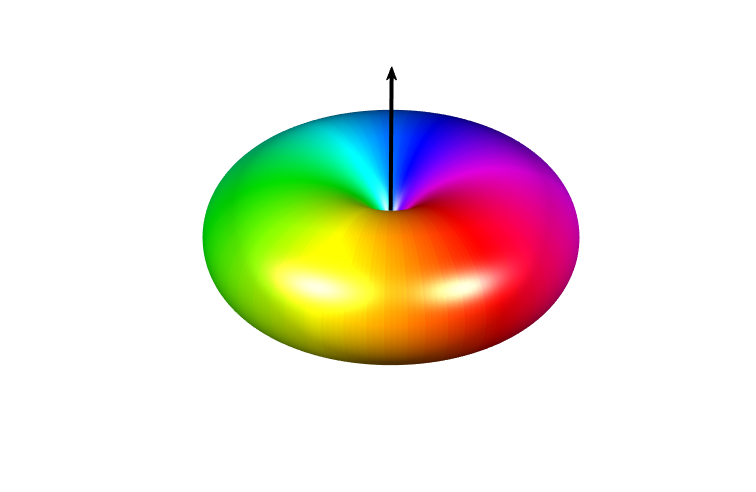
\includegraphics[width=\textwidth]
        {gfx/ch-groundStateSymmetries/FM-spherical.png}
        \caption{\(\zeta^\mathrm{FM}={(1, 0, 0)}^T\)}
    \end{subfigure}
    \begin{subfigure}{0.49\textwidth}
        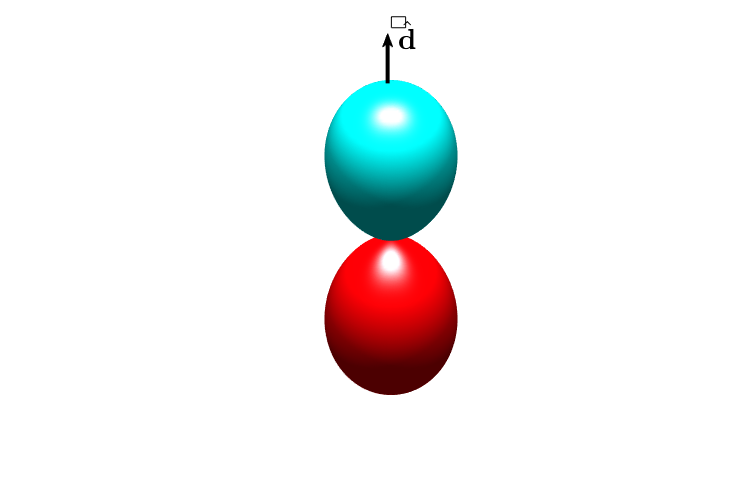
\includegraphics[width=\textwidth]
        {gfx/ch-groundStateSymmetries/polar-spherical.png}
        \caption{\(\zeta^\mathrm{P}={(0, 1, 0)}^T\)}
    \end{subfigure}
    \caption{Spherical harmonics of polar and FM ground states
    here.
    (a): The spin-1 ferromagnetic ground state with
    \(\zeta^\mathrm{FM}={(1, 0, 0)}^T\).
    The black arrow represents the direction of the condensate magnetisation.
    (b): The spin-1 polar ground state with
    \(\zeta^\mathrm{P}={(0, 1, 0)}^T\).
    The arrow represents the orientation of the nematic director,
    \(\hat{\vb{d}}\).\label{fig: spin-1-spherical-harmonics}
    \textcolor{red}{Add colour bar. Fix weird thing above polar spherical
    harmonic.}}
\end{figure}

\subsection{Majorana representation}
An alternative description to visualising the symmetries of spinor BECs is
through the use of the Majorana representation~\cite{Majorana1932,Bloch1945},
where a spin-\(f\) system can be represented as \(2f\) points on the Bloch
sphere.
The points on the sphere are numerically calculated as the \(2f\) roots
\(z_j\) of the polynomial equation
\begin{equation}
    P^{(f)}(z) = \sum_{\alpha = 0}^{2f}
    \sqrt{\mqty(2f \\ \alpha)}\zeta_{f-\alpha}^*z^\alpha=0,
\end{equation}
where each root represents a stereographic mapping
\(z_j=\tan(\theta/2)e^{i\phi}\) of the spherical coordinates \((\theta, \phi)\).
For spin-1, the polynomial becomes
\begin{equation}
    P^{(1)}(z) = \zeta_1^*z^2+\sqrt{2}\zeta_0^*z+\zeta_{-1}^*.
\end{equation}
The disadvantage of this representation is that one is not able to see the
condensate phase.

The Majorana representations for the states shown in
Fig.~\ref{fig: spin-1-spherical-harmonics} are shown in
Fig.~\ref{fig: spin-1-majorana}.
\begin{figure}
    \centering
    \includegraphics[scale=0.5]{example-image}
    \caption{\label{fig: spin-1-majorana}Majorana representations go here.}
\end{figure}

\section{Spin-2}
The interacting Hamiltonian for the spin-2 system is given by
\begin{equation}
    E_\mathrm{int} = \int c_0n^2 + c_1|\vb{F}|^2+c_2|A_{20}|^2.
\end{equation}
As before, the density remains fixed for any normalised ground state and so
different ground states arise from the competition between the spin-
and singlet-dependent interaction strengths.
If we first consider \(c_1, c_2 < 0\), then the energy functional is minimised
when both the spin density and singlet-duo amplitude are maximised: \(|F|=2n\)
and \(|A_{20}|=n/5\).
Such a state is ferromagnetic with spin \(|F|=2n\), which we call the FM-2
state.
There also exists a ferromagnetic state with spin \(|F|=n\), denoted as the FM-1
state.
This state is not the ground state since the FM-2 state has lower
energy.
However, it should be noted that the FM-1 state can remain stable in
certain situations, such as in the cores of vortices (see
Chapter~\ref{chap: spin-2}).
The representative spinors for the spin-2 ferromagnetic states have the form
\begin{equation}
    \zeta^\mathrm{FM-2} = \mqty(1 \\ 0 \\ 0 \\ 0 \\ 0), \qquad
    \zeta^\mathrm{FM-1} = \mqty(0 \\ 1 \\ 0 \\ 0 \\ 0).
\end{equation}
As in the spin-1 case, the energy of a given spinor in the absence of a magnetic
field is degenerate following the application of a global \(U(1)\) phase and an
\(SO(3)\) spin rotation.
In a spin-2 system, a general spin rotation is instead represented as a
\(5\times 5\) matrix of the form
\begin{equation}
    U(\alpha, \beta, \gamma) = \mqty(
        e^{-2i(\alpha + \gamma)}C^4 & -2e^{-i(2\alpha+\gamma)}C^3S 
        & \sqrt{6}e^{-2i\alpha}C^2S^2 & -2e^{-i(2\alpha-\gamma)}CS^3
        & e^{-2i(\alpha + \gamma)}S^4
    ),
\end{equation}

\subsection{Spherical harmonic representation}

\subsection{Majorana representation}

\subsection{Ground states in a uniform system}

\subsection{Ground states with conserved magnetisation}

\subsection{Stationary solutions}

\section{Vortices in spinor BECs}

\subsection{Spin-1}
\subsubsection{The spin-1 half-quantum vortex}

\subsection{Spin-2}

\subsubsection{The ferromagnetic phase}
\subsubsection{The cyclic phase}
\subsubsection{The uniaxial-nematic phase}
\subsubsection{The biaxial-nematic phase}
